%----------------------------------------------------------------------------------------
%	PACKAGES AND DOCUMENT CONFIGURATIONS
%----------------------------------------------------------------------------------------
\documentclass[11pt]{article}
\usepackage{amsmath} % Required for some math elements
\usepackage[usenames,dvipsnames]{xcolor}
\usepackage{lipsum} 
\usepackage{cite}
\usepackage{graphicx} % Required for the inclusion of images
\usepackage{algorithmic}
\usepackage{array}
\usepackage{bookmark}
\usepackage{listings}
\usepackage{amssymb}
\usepackage{enumitem}
\usepackage[margin=24mm]{geometry}
\usepackage[caption=false, font=footnotesize]{subfig}
\usepackage{multirow}
\usepackage[active,tightpage]{preview}
\usepackage{hyperref} 



\renewcommand{\PreviewBorder}{1in}
\newcommand{\Newpage}{\end{preview}\begin{preview}}

\newlist{steps}{enumerate}{1}
\setlist[steps, 1]{label = Step \arabic*:}

\hypersetup{ %color attributes of citation, link, etc.
    colorlinks=true,
    linkcolor=blue,
    filecolor=gray,      
    urlcolor=blue,
    citecolor=blue,
}

 
\lstdefinelanguage{VHDL}{
   morekeywords=[1]{
     library,use,all,entity,is,port,in,out,end,architecture,of,
     begin,and,or,Not,downto,ALL
   },
   morekeywords=[2]{
     STD_LOGIC_VECTOR,STD_LOGIC,IEEE,STD_LOGIC_1164,
     NUMERIC_STD,STD_LOGIC_ARITH,STD_LOGIC_UNSIGNED,std_logic_vector,
     std_logic
   },
   morecomment=[l]--
}
\definecolor{keyword}{rgb}{0,0.3,0.7}
\definecolor{STD}{rgb}{0.9,0.0,0.7}
\definecolor{comment}{rgb}{0.0,0.6,0.1}

\lstdefinestyle{vhdl}{
   language     = VHDL,
   basicstyle   = \footnotesize\ttfamily,
   keywordstyle = [1]\color{keyword}\bfseries,
   keywordstyle = [2]\color{STD}\bfseries,
   commentstyle = \color{comment}
   breaklines=true,                % sets automatic line breaking
   tabsize=3		                   % sets default tabsize to 2 spaces
}


\newcommand{\matlab}{\textsc{Matlab }} %very important and totally necessary addition

\newcommand\Item[1][]{%
  \ifx\relax#1\relax  \item \else \item[#1] \fi
  \abovedisplayskip=0pt\abovedisplayshortskip=0pt~\vspace*{-\baselineskip}}
  %----------------------------------------------------------------------------------------
%	DOCUMENT INFORMATION
%----------------------------------------------------------------------------------------
 
\title{ECEN302 : Integrated Digital Electronics \\ Lab 4 Submission}
\author{Daniel Eisen : 300447549}
\date{\today}


\begin{document}
\begin{preview}
\maketitle
%----------------------------------------------------------------------------------------
%	DOCUMENT CONTENT
%----------------------------------------------------------------------------------------
\section{Objectives}
The purpose of these lab exercises was to explore and utilise Finite State Machine (FSM) modelling in implementing a solution in HDL. Specifically it aims to solve to distinct problems with each a Mealy and a Moore FSM, exploring the differences in design, implementation and function/behaviours; both advantages and downsides.

\section{Methodology}
  \subsection{Mealy}
  Mealy State Machines change their output based on their current input and present state, rather than just the present state. This means that the output can be asynchronous to the clock as the input can be external and independent from the state change clock. Due the lack of absolute reliance of state-based output they can generally have less states. However, less states doesn't always mean simpler to implement. 

  This was shown with these exercises as each tasks was better suited to the other kind of FSM. 

  \lstinputlisting[language = VHDL]{inc/FSM_Mealy1.vhd}
  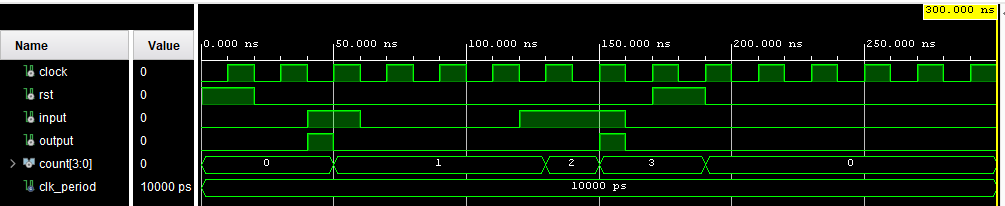
\includegraphics[width=\textwidth]{inc/mealy}
  \subsection{Moore}
  Moore machines only change states on the clock edge, and because of this predictability they can be safer to use, simply to design but can generally lead to more states and indeed real world circuitry to implementing. Due to this it is possible for a Mealy machine to operate faster, but you loose the synchronicity.  

  In this case I initially design the diagram with 6 states but after spending some time could collapse 2 pairs into each other to form the below simplification. But a mealy machine could possibly do it in 2 states and rely more heavily on the current input.

  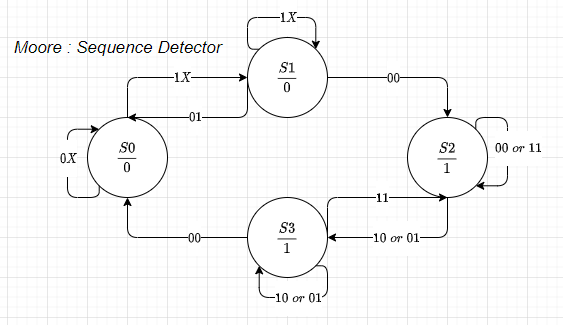
\includegraphics[width=\textwidth]{inc/moore_diagram}
  \lstinputlisting[language = VHDL]{inc/FSM_Moore.vhd}
  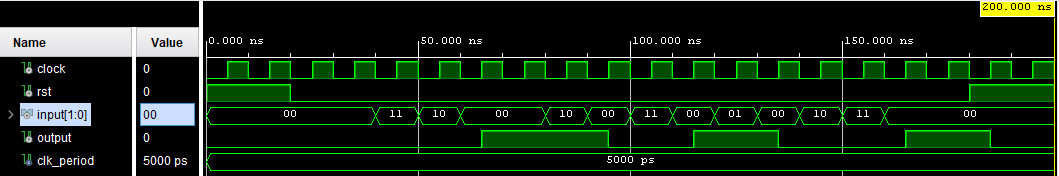
\includegraphics[width=\textwidth]{inc/moore}
  
  \section*{Concluding}
  While I see the advantages of mealy I much preferred the design and implementation of a Moore design as it made \textit{more} intuitive sense to me and generally took less time.
\end{preview}
\end{document}